\subsection{Query Evaluations}
\label{subsec:query-eval}
\textsc{Synopsis} incorporates support for user-defined queries that are evaluated over the distributed sketch.  Queries can be specified by the user in a SQL-like format or with JSON-based key-value descriptions similar to GraphQL~\cite{graphql}. Exact-match, range-based, and summarization queries are all supported over spatiotemporal bounds and individual feature values. Depending on scaling operations and the spatial scope of the queries, evaluations are carried out on one or more sketchlet instances. Information on the placement of sketchlets in the system and their corresponding feature scopes is maintained at each node in a Geohash prefix tree, with changes propagated through the network in an eventually-consistent manner as data is ingested and scaling maneuvers occur.

The entry point for these queries, called the \emph{conduit}, may be any of the nodes comprising the distributed sketch. During query evaluations, the first step is to identify the set of \textsc{Synopsis} nodes that are relevant to the query. The conduit consults its prefix tree to locate nodes based on spatial, chronological, and feature constraints specified by the user. After this process is complete, the conduit forwards the queries on to the nodes for evaluation and supplies the client with a list of nodes that will respond to the query. As queries execute, results are streamed back to the client where they are merged by the client API. This strategy ensures that I/O and processing activities are interleaved on the client side.

Our distributed prefix tree enables query evaluations during both scaling in and out. When a conduit attempts to forward a query to a node that is undergoing a scaling operation, the request will be redirected to the destination's parent node. This process can continue recursively up through the network, ensuring queries will reach their final destination.

\subsection{Query Types}
\textsc{Synopsis} queries can be discrete or continuous. Unlike discrete queries that are evaluated once, continuous queries are evaluated periodically or when observations become available. We classify queries -- discrete or continuous -- supported by \textsc{Synopsis} into six broad categories:

\begin{description}[leftmargin=*]
	\item[Relational Queries] describe the feature space in the context of our hierarchical graphs and may target ranges of values under certain conditions. For example, ``What is the relationship between temperature and humidity during July in Alaska, USA, when precipitation was greater than 1 centimeter?'' These queries return a subset of the overall sketch that includes other matching feature values as well.% Subsketches may be manipulated and inspected on the client side, and then reused in subsequent queries to request more detail or broaden the query scope. Relational queries can optionally return statistical metadata stored in the leaf nodes of the graph; this is also supported by our statistical query functionality.

\item[Statistical Queries] allow users to explore statistical properties of the observational space by retrieving portions of the metadata stored in the leaf nodes of the sketch. For example, users can retrieve and contrast correlations between any two features at different geographic locations at the same time. Alternatively, queries may contrast correlations between different features at different time ranges at the same geographic location. Statistical queries also support retrieval of the mean, standard deviation, and feature outliers based on Chebyshev's inequality \cite{knuth1968art}.

\item[Density Queries] support analysis of the distribution of values associated with a feature over a particular spatiotemporal scope. These include kernel density estimations, estimating the probability of observing a particular value for an observation, and determining the deciles and quartiles for the observed feature.% Kernel density estimations can request the function itself, an integral over a range of values, or the probability of a single value.

\item[Set Queries] target identification of whether a particular combination of feature values was observed, estimating the cardinality of the dataset, and identifying the frequencies of the observations. Each type of set query requires a particular data structure, with instances created across configurable time bounds (for instance, every day). Set membership is determined using space-efficient bloom~filters~\cite{bloom1970space}, while cardinality (number of distinct elements) queries are supported by the HyperLogLog~\cite{flajolet2007hyperloglog} algorithm. Finally, cardinality (number of distinct elements) queries are supported by the HyperLogLog~\cite{flajolet2007hyperloglog} algorithm. 

%To determine set membership, we use Bloom filters may produce false positives, but never false negatives. Besides returning a \texttt{true} or \texttt{false} result to the user, membership queries also include the probability of the answer being a false positive.  Set HyperLogLog is able to estimate cardinality with high accuracy and low memory consumption. Finally, observation frequencies are provided by the count-min data structure \cite{cormode2005improved}. Count-min is structurally similar to a bloom filter, but can be used to estimate the frequency of values within a particular error band. Frequency queries are accompanied by their associated confidence intervals and relative error.

\item[Inferential Queries]
Inferential queries enable spatiotemporal forecasts to be produced for a particular feature (or set of features). Discrete inferential queries leverage existing information in the distributed sketch to make predictions; aggregate metadata stored in the leaves of the graph can produce two-dimensional regression models that forecast new outcomes across each feature type when an independent variable of interest changes. 

%In their continuous form, inferential queries are backed by machine learning models that are \emph{installed} for a particular time window and can be trained using either the sketch or new, full-resolution values as they arrive. Continuous inferential queries can stream predictions back to the client on a regular interval, or a subsequent query can reference a particular model and parameterize it to make a single prediction. Our current implementation of \textsc{Synopsis} supports multiple linear regression, but our machine learning interface allows new models to be plugged into the system at run time.

\item[Synthetic Data Queries] allow users to request the system to generate representative datasets based on the distributions stored in the sketch. Synthetic data is generated in an online fashion by sampling from the underlying distributions and then streamed to client applications for analytics. The size of the dataset may also be specified; for instance, 10\% of the volume of the original data points.
\end{description}

\subsection{Query Evaluation Performance}
To evaluate distributed query performance, we executed several representative workloads across a variety of sketchlet sizes. These queries were separated into two groups: metadata lookups and graph retrievals. Metadata lookups include density queries, set queries, and statistical queries, while graph retrievals request targeted portions of the overall feature space as a graph.  Note that while metadata lookups do not return a graph structure to the client, they still require a graph traversal to resolve. In general, graph retrievals consume more processing time due to their high serialization and I/O costs.

Figure~\ref{fig:dist-query} demonstrates the end-to-end efficiency of the query evaluations over the distributed sketch.
Cumulative query throughput and latencies were measured with varying numbers of concurrent query \emph{funnels}.
A query \emph{funnel} continuously generates and dispatches random queries at their maximum possible rate to stress test the system and saturate its capacity; for instance, a query could request summary statistics or feature relationships when the temperature is between 20 to 30 degrees, humidity is above 80\%, and the wind is blowing at 16 km/h.
These randomized queries fluctuated in both the ranges of values and spatial scope, resulting in high variability in the number of \textsc{Synopsis} nodes required to resolve the query as well as the depth and breadth of the required graph traversals.

\begin{figure*}
    \centerline{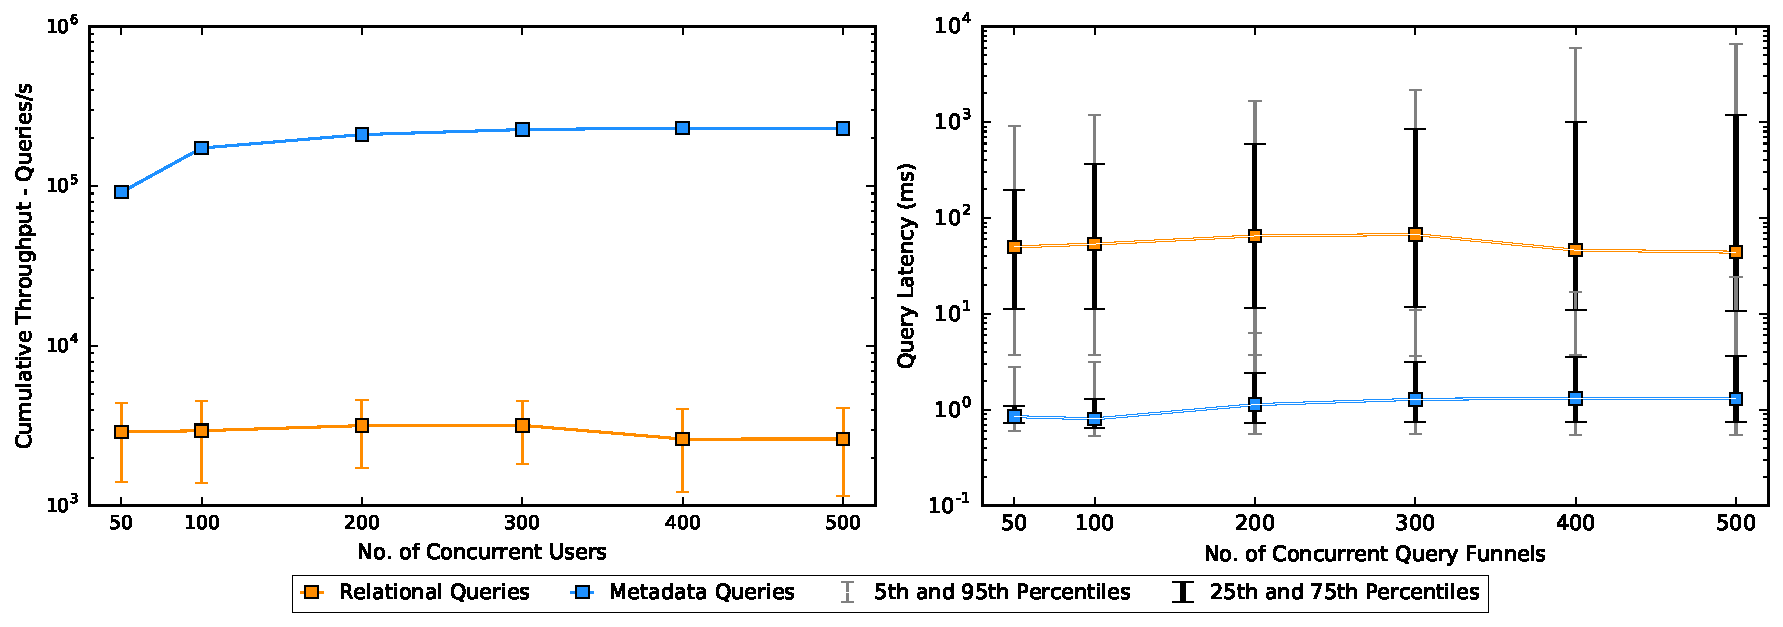
\includegraphics[width=\linewidth]{figures/query_benchmark_both.pdf}}
    \caption{Distributed Query Evaluation Performance. Variation of cumulative throughput and latency against the number of concurrent query funnels in a 40 node \textsc{Synopsis} cluster.}
    \label{fig:dist-query}
\end{figure*}

Table~\ref{tbl:query-times} outlines the local sketchlet traversal times for both evaluation types on a single node, and also includes results that combine the two types (retrieving a graph that also includes metadata). In general, metadata lookups require less processing time. While graph lookups take longer to complete, it is worth noting that varying the geographical scope across sketchlet sizes from 5km to 800km did not result in a proportionate increase in processing time. Overall, the sketch is able to satisfy our goal of low-latency query evaluations for each query type.

\begin{table}[h!]
    \renewcommand{\arraystretch}{1.4}
    \caption{Local sketchlet evaluation times for each query type (averaged over 1000 iterations).}
    \label{tbl:query-times}
    \begin{center}
        \begin{tabular}{|l|c|c|}
            \hline
            \textbf{Query Type}      & \textbf{Eval. (ms)} & \textbf{Std. Dev.} \\
            \hline
            Density                  & 0.007                    & 0.005 \\
            \hline
            Set Cardinality          & 0.154                    & 0.088 \\
            \hline
            Set Frequency            & 0.036                    & 0.019 \\
            \hline
            Set Membership           & 0.015                    & 0.009 \\
            \hline
            Statistics               & 0.002                    & 0.001 \\
            \hline
            \hline
            Graph Only (5 km)        & 46.357                   & 1.287 \\
            \hline
            Graph + Meta (5 km)      & 40.510                   & 6.937 \\
            \hline
            Graph + Meta (25 km)     & 47.619                   & 6.355 \\
            \hline
            Graph + Meta (800 km)    & 53.620                   & 6.818 \\
            \hline
        \end{tabular}
    \end{center}
\end{table}
